\documentclass{article}

\usepackage[letterpaper,top=2cm,bottom=2cm,left=3cm,right=3cm,marginparwidth=1.75cm]{geometry}

\usepackage{booktabs}
\usepackage{tabularx}
\usepackage{hyperref}
\usepackage{float}
\usepackage{graphicx}
\usepackage{color}
\usepackage{soul}
\hypersetup{
    colorlinks=true,
    urlcolor=cyan
    }

\title{SE 3XA3: Development Plan}

\author{Group \#10
        \\Lab: L03
		\\ Aamina Hussain, hussaa54
		\\ Jessica Dawson, dawsor1
		\\ Fady Morcos, morcof2
}

\date{}

%\input{../Comments}

\begin{document}
\newpage
\maketitle
\newpage

\begin{table}[h!]
\caption{Revision History} \label{TblRevisionHistory}
\begin{tabularx}{\textwidth}{llX}
\toprule
\textbf{Date} & \textbf{Developer(s)} & \textbf{Change}\\
\midrule
Feb 4, 2022 & Jessica Dawson, Aamina Hussain, and Fady Morcos & First version\\
\color{red} Apr 11, 2022 & \color{red} Aamina Hussain & \color{red}Updated Section 6, Added Section 9 Project Review\\
\bottomrule
\end{tabularx}
\end{table}

\newpage


\maketitle

This document contains the development plan for recreating a random abstract art generator. This plan will ensure the developers communicate properly, are consistent, and follow the project schedule.

\section{Team Meeting Plan}

The team shall meet twice a week during labs:
\begin{itemize}
    \item Mondays, 9:30 am to 11:30 am
    \item Wednesdays, 9:30 am to 11:30 am
\end{itemize}
The team shall also meet at least once a week outside of labs. The location, day, time, and duration of this meeting will be decided weekly based on convenience and necessity.

\section{Team Communication Plan}

The team will communicate using the Microsoft Teams chat. This chat will be used to schedule weekly meetings and any further discussions that were not finalized during the in-person labs.

\section{Team Member Roles}

The team member roles are:
\begin{itemize}
    \item Developer: Aamina Hussain, Fady Morcos, Jessica Dawson
    \item Scribe (records/transcribes what occurs during meetings): Aamina Hussain
    \item Communicator (asks the supervisors (the TAs) questions that the team has): Fady Morcos
    \item Submitter (makes sure documents are finalized and submitted before the deadline): Jessica Dawson
\end{itemize}

\section{Git Workflow Plan}

\begin{figure}[H]
    \centering
    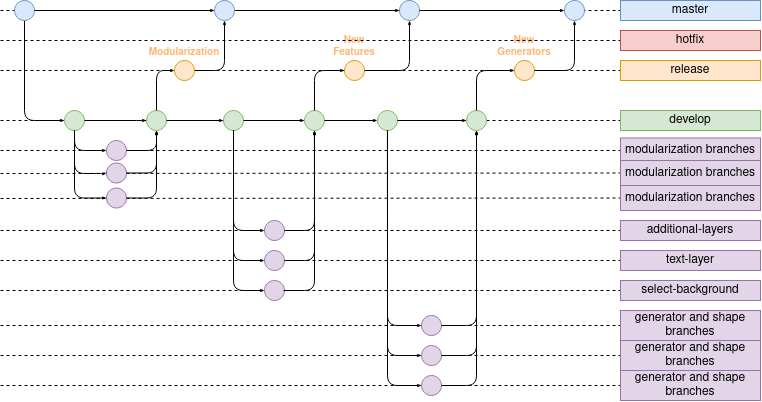
\includegraphics[width=0.9\textwidth]{git-workflow.png}
    \caption{git workflow}
\end{figure}

Git Branches:

\begin{itemize}
    \item master: for production ready releases, each release will be tagged with a version number
    \item develop: main development branch, for unstable nightly commits
    \item release: for cleanup before a release
    \item hotfix: for fixing any bugs found in a production release
    \item modularization branches: a set of feature branches for modularizing the code architecture, what these will look like will depend on a more indepth analysis of the code and what needs to be reworked
    \item addition-layers: feature branch for adding extra drawing layers to the program
    \item text-layer: feature branch for adding a layer that writes text on top of the art
    \item select-background: feature branch for allowing the user to pick the background color
    \item generator and shape branches: a set of feature branches each one adding a new generator or shape, what these will look like will depend on what new generators and shapes we decide to add
\end{itemize}

We will use a gitlab issue board to keep track of tasks with an open list for unassigned tasks, a board for each team member for their assigned tasks, and a closed board for finished tasks. Labels will be used to mark these tasks and associated merge requests.\newline

Task Labels:

\begin{itemize}
    \item bug: for bugfixes
    \item enhancement: for reworking code without adding features
    \item feature: for adding a feature to the code
    \item available: for an unassigned issue
    \item todo: for an assigned issue that has yet to be started
    \item in-progress: for an issue currently being worked on
    \item merge-ready: for an issue ready to be merged
    \item completed: for a fully merged and completed issue
\end{itemize}

Milestones will be used to track the completion of and group issues related to different section of our workflow plan:

\begin{itemize}
    \item modularization: for tracking the completion of the first set of tasks related to the modularization of the code
    \item additional layers: for tracking the development of the additional layers features
    \item text layer: for tracking the development of the text layer features
    \item select background: for tracking the development of the select background color feature
    \item generators and shapes: for tracking the development of new generators and shapes
\end{itemize}

\section{Proof of Concept Demonstration Plan}

None of the required python library are difficult to install for this project. All of the modules can easily be installed from a command line using pip install quickly. However, this leads to portability being a bit concerning since the user will have to install these libraries in order to run the program. The proof of concept demonstration will consist of us running the Python program where we modularize the original code and add at least one new feature. This will create an interface where the user can choose different options for the abstract art they want generated. This demo will prove that we are capable of creating the core or bulk of the project.

\section{Technology}

The program will be written using the Python programming language. One of the main Python libraries we will be using is Pygame. The code will be written using an IDE called PyCharm. \st{The team will use the testing framework Pytest to test our program.} \color{red} Latex will be used for generating most of the documentation. The MIS document will be generated using Doxygen.\\

\noindent \#\#COMMENT: We realized that it would not be logical to test our code using an automated or unit testing framework due to the nature of the program. This program can only be tested by actually viewing the generated output, so for this reason we decided to forgo automated testing and use a manual testing approach to test our program.\color{black}

\section{Coding Style}

The Google python style guide will be used: \url{https://google.github.io/styleguide/pyguide.html}

\section{Project Schedule}

Please refer to
\href{https://gitlab.cas.mcmaster.ca/3xa3-l3-g10/3xa3-l3-g10/-/tree/main/ProjectSchedule}{this link}.

\section{Project Review}
\color{red} After the Revision 1 Demonstration, we are considering this project to be successfully completed. Despite the short period of time we had for this project, we completed all the objectives we had set at the start. This includes all objectives we had pertaining to the project's documentation, as well as objectives for the program code.\\

\noindent The success of the project can be attributed to the planning and constant communication of the team members. This allowed each member to be aware of their exact tasks and when those tasks had to be completed. We planned for lengthy tasks to be completed ahead of time in case those tasks ended up taking longer to complete than planned. We were also fully open to meeting outside of our usual meet-up times if necessary.\\

\noindent An area of improvement for our team is using git to its full extent. There was a bit of a learning curve for us when it came to using git, and instead of each working on separate branches, we usually messaged and let everyone know when we were pushing an update to the main branch. The workflow would have been smoother if we had full knowledge of the functionalities of git and actually used them.

\end{document}
